\documentclass{standalone}
\usepackage{pgfplots}
\pgfplotsset{compat=1.13}
\usepackage{amsmath}

\begin{document}

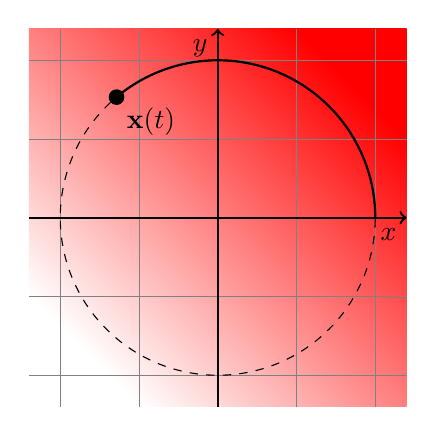
\begin{tikzpicture}
    \shade[shading=axis, top color=red, shading angle=-45] (-2.4,-2.4) rectangle (2.4,2.4);
    \draw[step=1cm,gray,very thin] (-2.4,-2.4) grid (2.4,2.4);
    \draw[thick,->] (-2.4,0) -- (2.4,0) node[anchor=north east]{\(x\)};
    \draw[thick,->] (0,-2.4) -- (0,2.4) node[anchor=north east]{\(y\)};
    \draw[dashed] (0,0) circle (2);
    \draw[thick] (2,0) arc [start angle=0, end angle=130, radius=2] node[circle,fill,inner sep=2pt]{} node[anchor=north west]{\(\mathbf{x}(t)\)};
\end{tikzpicture}

\end{document}